% This is a LaTeX thesis template for Monash University.
% to be used with Rmarkdown
% This template was produced by Rob Hyndman
% Version: 6 September 2016

\documentclass[doubleside,doublespace]{aucklandthesis}

%%%%%%%%%%%%%%%%%%%%%%%%%%%%%%%%%%%%%%%%%%%%%%%%%%%%%%%%%%%%%%%
% Add any LaTeX packages and other preamble here if required
%%%%%%%%%%%%%%%%%%%%%%%%%%%%%%%%%%%%%%%%%%%%%%%%%%%%%%%%%%%%%%%

\author{Marie Curie}
\title{Thesis title}
\degrees{B.Sc. (Hons), The University of Auckland}
\def\degreetitle{Doctor of Philosophy}
% Add subject and keywords below
\hypersetup{
     %pdfsubject={The Subject},
     %pdfkeywords={Some Keywords},
     pdfauthor={Marie Curie},
     pdftitle={Thesis title},
     pdfproducer={Bookdown with LaTeX}
}


\bibliography{thesisrefs}

\begin{document}

\pagenumbering{roman}

\titlepage

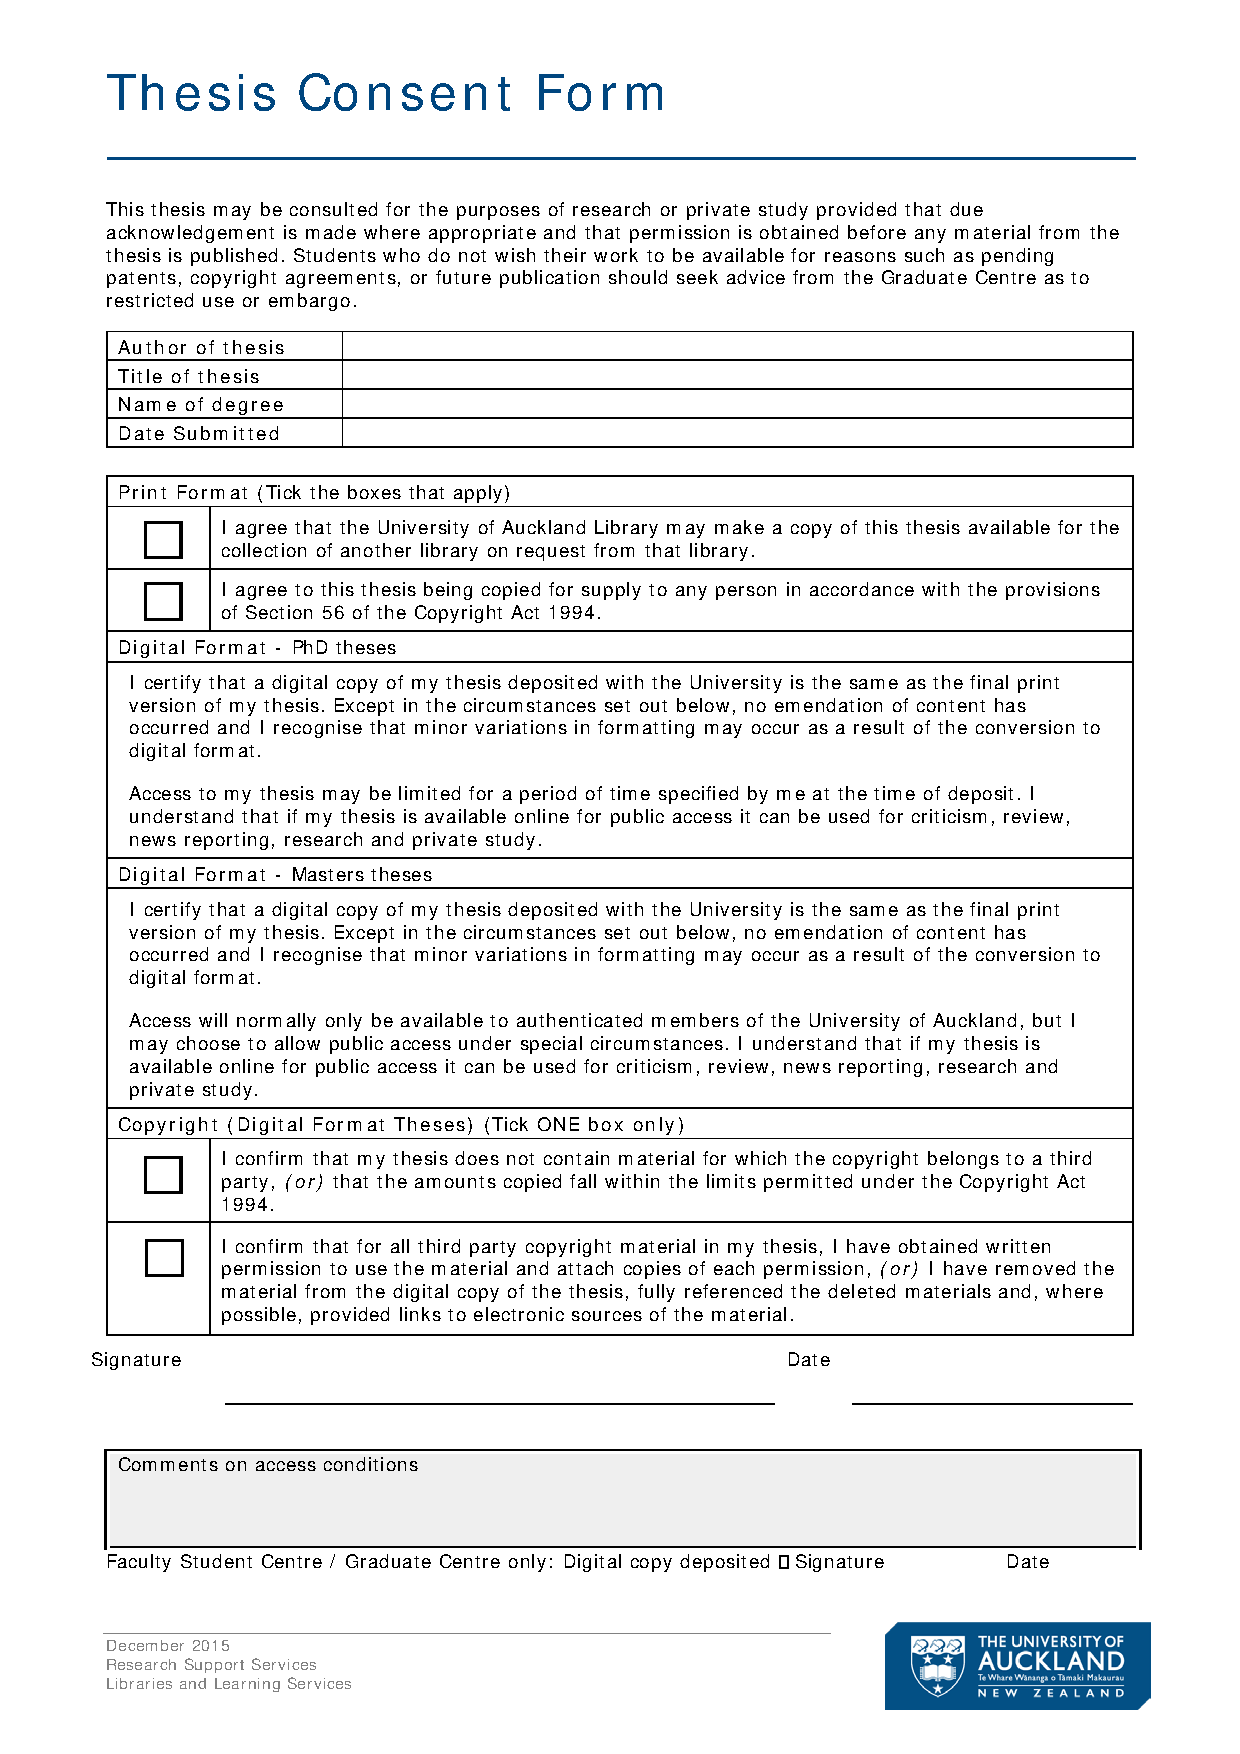
\includepdf{thesisconsent.pdf}

\hypertarget{abstract}{%
\chapter*{Abstract}\label{abstract}}
\addcontentsline{toc}{chapter}{Abstract}

The abstract should outline the main approach and findings of the thesis and must not be more than 500 words.

\cleardoublepage

\hypertarget{acknowledgements}{%
\chapter*{Acknowledgements}\label{acknowledgements}}
\addcontentsline{toc}{chapter}{Acknowledgements}

I would like to thank my pet goldfish for \dots

\cleardoublepage

\begingroup
\setstretch{1.2}\tighttoc\doublespacing
\endgroup

\clearpage

\phantomsection 
\addcontentsline{toc}{chapter}{List of Figures}

\begingroup
\setstretch{1.2}\listoffigures\doublespacing
\endgroup

\clearpage

\phantomsection 
\addcontentsline{toc}{chapter}{List of Tables}

\begingroup
\setstretch{1.2}\listoftables\doublespacing
\endgroup

\cleardoublepage

\pagenumbering{arabic}\setcounter{page}{0}

\hypertarget{ch:intro}{%
\chapter{Introduction}\label{ch:intro}}

This is where you introduce the main ideas of your thesis, and an overview of the context and background.

In a PhD, Chapter 2 would normally contain a literature review. Typically, Chapters 3--5 would contain your own contributions. Think of each of these as potential papers to be submitted to journals. Finally, Chapter 6 provides some concluding remarks, discussion, ideas for future research, and so on. Appendixes can contain additional material that don't fit into any chapters, but that you want to put on record. For example, additional tables, output, etc.

\hypertarget{rmarkdown}{%
\section{Rmarkdown}\label{rmarkdown}}

In this template, the rest of the chapter shows how to use Rmarkdown. The big advantage of using Rmarkdown is that it allows you to include your R code directly into your thesis, to ensure there are no errors in copying and pasting, and that everything is reproducible. It also helps you stay better organized.

For details on using \emph{R Markdown} see \url{http://rmarkdown.rstudio.com}.

\hypertarget{data}{%
\section{Data}\label{data}}

Included in this template is a file called \texttt{sales.csv}. This contains quarterly data on Sales and Advertising budget for a small company over the period 1981--2005. It also contains the GDP (gross domestic product) over the same period. All series have been adjusted for inflation. We can load in this data set using the following command:

\begin{Shaded}
\begin{Highlighting}[]
\NormalTok{sales }\OtherTok{\textless{}{-}} \FunctionTok{ts}\NormalTok{(}\FunctionTok{read.csv}\NormalTok{(}\StringTok{"data/sales.csv"}\NormalTok{)[,}\SpecialCharTok{{-}}\DecValTok{1}\NormalTok{], }\AttributeTok{start=}\DecValTok{1981}\NormalTok{, }\AttributeTok{frequency=}\DecValTok{4}\NormalTok{)}
\end{Highlighting}
\end{Shaded}

Any data you use in your thesis can go into the data directory. The data should be in exactly the format you obtained it. Do no editing or manipulation of the data outside of R. Any data munging should be scripted in R and form part of your thesis files (possibly hidden in the output).

\hypertarget{figures}{%
\section{Figures}\label{figures}}

Figure \ref{fig:deaths} shows time plots of the data we just loaded. Notice how figure captions and references work. Chunk names can be used as figure labels with \texttt{fig:} prefixed. Never manually type figure numbers, as they can change when you add or delete figures. This way, the figure numbering is always correct.

\begin{figure}
\centering
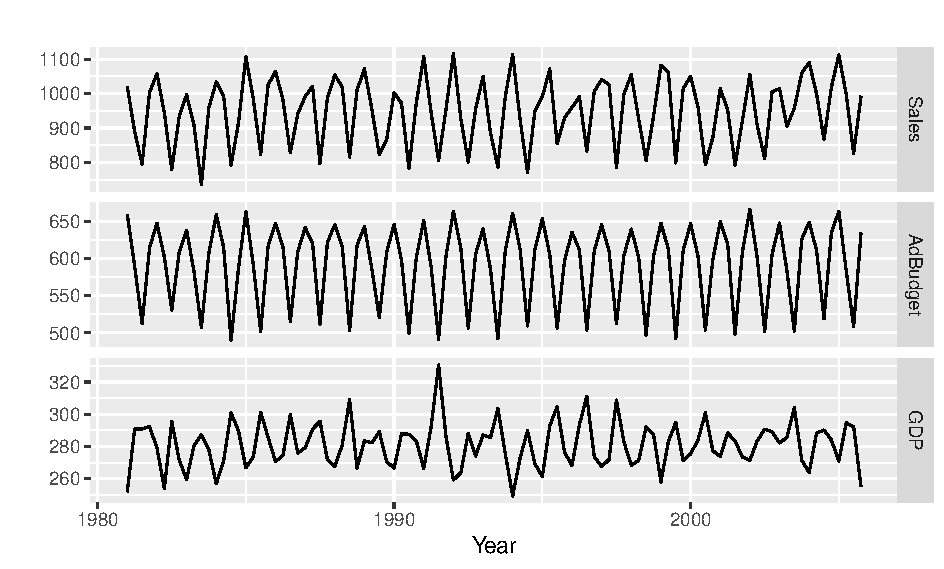
\includegraphics{thesis_files/figure-latex/deaths-1.pdf}
\caption{\label{fig:deaths}Quarterly sales, advertising and GDP data.}
\end{figure}

\hypertarget{results-from-analyses}{%
\section{Results from analyses}\label{results-from-analyses}}

We can fit a dynamic regression model to the sales data.

If \(y_t\) denotes the sales in quarter \(t\), \(x_t\) denotes the corresponding advertising budget and \(z_t\) denotes the GDP, then the resulting model is:
\begin{equation}
  y_t - y_{t-4} = \beta (x_t-x_{t-4}) + \gamma (z_t-z_{t-4}) + \theta_1 \varepsilon_{t-1} + \Theta_1 \varepsilon_{t-4} + \varepsilon_t
\end{equation}
where
\(\beta = 2.28\),
\(\gamma = 0.97\),
\(\theta_1 = NA\),
and
\(\Theta_1 = -0.90\).

\hypertarget{tables}{%
\section{Tables}\label{tables}}

Let's assume future advertising spend and GDP are at the current levels. Then forecasts for the next year are given in Table \ref{tab:salesforecasts}.

\begin{verbatim}
## Warning in sprintf(str, x, ...): one argument not used by format '\toprule
## Point Forecast & Lo 80 & Hi 80 & Lo 95 & Hi 95 \\
## \midrule'

## Warning in sprintf(str, x, ...): one argument not used by format '\toprule
## Point Forecast & Lo 80 & Hi 80 & Lo 95 & Hi 95 \\
## \midrule'
\end{verbatim}

\begin{table}[ht]
\begin{center}
\begin{tabular}{lllll}
\toprule
Point Forecast & Lo 80 & Hi 80 & Lo 95 & Hi 95 \\
\midrule
1000.2 &  947.7 & 1052.7 & 919.9 & 1080.5 \\
1013.1 &  959.3 & 1066.8 & 930.9 & 1095.3 \\
1076.7 & 1022.9 & 1130.6 & 994.4 & 1159.0 \\
1003.5 &  949.7 & 1057.4 & 921.2 & 1085.8 \\
\bottomrule
\end{tabular}
\caption{Forecasts for the next year assuming Advertising budget and GDP are unchanged.}
\label{tab:salesforecasts}
\end{center}
\end{table}

Again, notice the use of labels and references to automatically generate Table numbers. In this case, we need to generate the label ourselves.

The \texttt{knitLatex} package is useful for generating tables from R output. Other packages can do similar things including the \texttt{kable} function in \texttt{knitr} which is somewhat simpler but you have less control over the result. If you use \texttt{knitLatex} to generate tables, don't forget to include \texttt{results="asis"} in the chunk settings.

\hypertarget{ch:litreview}{%
\chapter{Literature Review}\label{ch:litreview}}

This chapter contains a summary of the context in which your research is set.

Imagine you are writing for your fellow PhD students. Topics that are well-known to them do not have to be included here. But things that they may not know about should be included.

Resist the temptation to discuss everything you've read in the last few years. And you are not writing a textbook either. This chapter is meant to provide the background necessary to understand the material in subsequent chapters. Stick to that.

You will need to organize the literature review around themes, and within each theme provide a story explaining the development of ideas to date. In each theme, you should get to the point where your ideas will fit in. But leave your ideas to later chapters. This way it is clear what has been done beforehand, and what new contributions you are making to the research field.

All citations should be done using markdown notation as shown below. This way, your bibliography will be compiled automatically and correctly.

\hypertarget{sec:expsmooth}{%
\section{Exponential smoothing}\label{sec:expsmooth}}

Exponential smoothing was originally developed in the late 1950s \autocite{Brown59,Brown63,Holt57,Winters60}. Because of their computational simplicity and interpretability, they became widely used in practice.

Empirical studies by \textcite{MH79} and \textcite{Metal82} found little difference in forecast accuracy between exponential smoothing and ARIMA models. This made the family of exponential smoothing procedures an attractive proposition \autocite[see][]{CKOS01}.

The methods were less popular in academic circles until \textcite{OKS97} introduced a state space formulation of some of the methods, which was extended in \textcite{HKSG02} to cover the full range of exponential smoothing methods.

\appendix

\hypertarget{additional-stuff}{%
\chapter{Additional stuff}\label{additional-stuff}}

You might put some computer output here, or maybe additional tables.

Note that line 5 must appear before your first appendix. But other appendices can just start like any other chapter.


\begingroup
\setstretch{1.0}
\printbibliography[heading=bibintoc]
\endgroup



\end{document}
